% Supplementary material. Compile separately from main.tex.
% Do not append these pages to the CVPR submission PDF.

\documentclass[10pt,twocolumn,letterpaper]{article}
\usepackage[review]{cvpr}
\usepackage{graphicx}
\usepackage{placeins}
\usepackage{float}
\usepackage{amsmath}
\usepackage{amssymb}
\usepackage{booktabs}
\usepackage{multirow}
\usepackage{xcolor}
\usepackage{colortbl}
\definecolor{oursrow}{RGB}{232,242,250}

\definecolor{cvprblue}{rgb}{0.21,0.49,0.74}
\usepackage[pagebackref,breaklinks,colorlinks,allcolors=cvprblue]{hyperref}

\def\paperID{*****}
\def\confName{CVPR}
\def\confYear{2027}

\title{Supplementary Material\\HMamba-eMOT: Hypergraph Modulated State Updating in Mamba for RGB-Event Multi-Object Tracking}

\author{First Author\\
Institution1\\
Institution1 address\\
{\tt\small firstauthor@i1.org}
\and
Second Author\\
Institution2\\
First line of institution2 address\\
{\tt\small secondauthor@i2.org}
}

\begin{document}
\maketitle

This document collects material omitted from the main paper: the concept sketch, training and loss details, the inference search, and the hypergraph visualization.

\section{Concept Sketch}

\begin{figure*}[t]
  \centering
  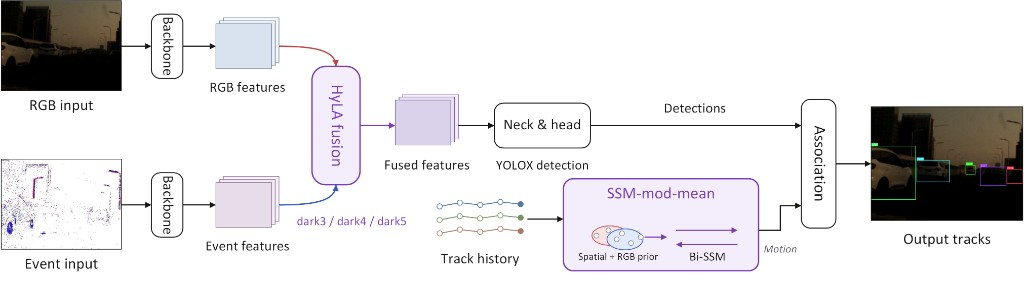
\includegraphics[width=\textwidth]{overall_framework_concept.png}
  \caption{Concept of the tracker. RGB and event frames pass through separate backbones and are fused by HyLA at blocks 1--3. A YOLOX neck and head turn the fused features into detections. Track history, together with a spatial and RGB prior, conditions a bidirectional state-space motion model. IoU association then writes the output tracks.}
  \label{fig:concept}
\end{figure*}

Figure~\ref{fig:concept} is the early sketch of the pipeline. The main paper uses the overview figure, which separates detection and motion into the two stages that are implemented.

\section{Loss and Training}

SimOTA assigns foreground anchors by a cost of classification and box overlap. $\mathcal{L}_{\mathrm{obj}}$ and $\mathcal{L}_{\mathrm{cls}}$ are binary cross-entropy with logits, on the objectness score and on the two class scores. The class target is the one-hot label scaled by the IoU of the matched box. $\mathcal{L}_{\mathrm{L1}}$ is an L1 penalty on the raw box regression. It is added only for the last nine epochs, the same epochs in which mosaic augmentation is turned off.

On FEMOT, the detector is YOLOX-X (depth $1.33$, width $1.25$), initialized from COCO and fine-tuned for $30$ epochs at batch size $24$ in FP16. The input resolution is $416\times416$ with multi-scale training, and mosaic augmentation is turned off for the last $9$ epochs. The learning rate is $0.001/128$ per image. The MambaTrack row in the FEMOT table is the sum-fusion dual-modal baseline on the same test split.

The motion model is initialized from a MambaTrack checkpoint trained on FEMOT for $30$ epochs with SGD and the Transformer learning-rate schedule at batch size $64$, using length-$12$ windows of annotated box differences and a Smooth-L1 loss on the next-box offset. It is then adapted for $10$ epochs with Adam at $5\times10^{-5}$, batch size $64$, gradient clipping at $1.0$, and no learning-rate schedule. A batch is skipped when its Smooth-L1 loss exceeds $1.0$. Appearance memories use EMA momentum $0.9$.

For DSEC-MOT, both detectors predict seven categories, are initialized from COCO, and are fine-tuned for $30$ epochs with batch size $24$ in FP16. Training uses $416\times416$ inputs, multi-scale augmentation, mosaic and mixup during the main schedule, and disables mosaic for the last $9$ epochs. The optimizer follows the YOLOX warm-cosine schedule. The MambaTrack baseline is trained for $10$ epochs with SGD and the Transformer learning-rate schedule on length-$12$ windows. Our tracker is then trained separately for $10$ epochs with Adam at $5\times10^{-5}$ and batch size $64$.

\section{Inference Search}

$T_{\mathrm{en}}$ is the minimum number of stored boxes before a track adopts the Mamba offset. The memory is initialized with the box that creates the track, so $T_{\mathrm{en}}=1$ runs Mamba on a history with no displacement, $T_{\mathrm{en}}=2$ waits for the second box, and larger values keep the last box until that many observations have been written. The reported model uses $T_{\mathrm{en}}=2$, which scores HOTA $45.50$, AssA $43.92$, and IDF1 $55.90$ at the final operating point. Entering Mamba at the first box scores HOTA $44.67$ under the sweep, because the scan is then driven by a zero-padded history. Waiting for a third or fourth box scores HOTA $44.19$ and $44.18$. After the second-stage cost has been set to $0.80$, $T_{\mathrm{en}}=2$ scores HOTA $44.94$, $T_{\mathrm{en}}=1$ scores $44.94$ with $65$ more identity switches, and $T_{\mathrm{en}}=3$ scores $44.74$.

\begin{table}[H]
  \centering
  \small
  \setlength{\tabcolsep}{3.2pt}
  \caption{Minimum memory length $T_{\mathrm{en}}$ before the Mamba offset is used. $T_{\mathrm{en}}=2$ is the reported model.}
  \label{tab:enable}
  \begin{tabular}{lccccc}
    \toprule
    $T_{\mathrm{en}}$ & HOTA & AssA & MOTA & IDF1 & IDSW \\
    \midrule
    1 & 44.67 & 41.93 & 50.92 & 54.21 & 3329 \\
    \rowcolor{oursrow}
    2 & 45.50 & 43.92 & 51.32 & 55.90 & 3220 \\
    3 & 44.19 & 41.27 & 49.98 & 53.27 & 3741 \\
    4 & 44.18 & 41.01 & 50.53 & 53.37 & 3617 \\
    \bottomrule
  \end{tabular}
\end{table}

From the default inference schedule, the largest accepted change among the remaining arguments is the second-stage cost, from $0.90$ to $0.80$ (HOTA $44.9$). Lowering the new-track score from $0.55$ to $0.45$ also reaches $44.9$, but IDSW rises to $3{,}749$, so $\tau_n$ stays $0.55$. With the second stage fixed at $0.80$ and $T_{\mathrm{en}}=2$, the next accepted change is $\tau_f=0.25$ (HOTA $45.2$), then the first-stage cost $0.75$ (HOTA $45.4$, still at $T_{\mathrm{lost}}=25$).

Around that checkpoint the search probes three arguments. Setting $T_{\mathrm{lost}}=20$ reaches HOTA $45.50$. At the same previous checkpoint, $\tau_f=0.28$ reaches $45.45$ and $\tau_1=0.78$ reaches $45.38$; both of those probes keep $T_{\mathrm{lost}}=25$. The search keeps $T_{\mathrm{lost}}=20$. A final check of the lost window, with every other argument held at the selected value, gives $45.25$ at $15$ frames and $45.39$ at $22$ frames (Table~\ref{tab:param}). The selected point is the best evaluated setting, and the lost-window neighbors lie within $0.3$ HOTA.

\begin{table}[H]
  \centering
  \small
  \setlength{\tabcolsep}{2.6pt}
  \caption{Lost-window check at the selected point. Every row uses $\tau_f=0.25$, $\tau_1=0.75$, $\tau_2=0.80$, $T_{\mathrm{en}}=2$ and $\tau_n=0.55$.}
  \label{tab:param}
  \begin{tabular}{lccccc}
    \toprule
    $T_{\mathrm{lost}}$ & HOTA & AssA & MOTA & IDF1 & IDSW \\
    \midrule
    15 & 45.25 & 43.48 & 51.39 & 55.75 & 3125 \\
    \rowcolor{oursrow}
    20 & 45.50 & 43.92 & 51.32 & 55.90 & 3220 \\
    22 & 45.39 & 43.66 & 51.31 & 55.65 & 3278 \\
    25 & 45.38 & 43.61 & 51.27 & 55.67 & 3307 \\
    \bottomrule
  \end{tabular}
\end{table}

\section{Hypergraph Visualization}

\begin{figure*}[t]
  \centering
  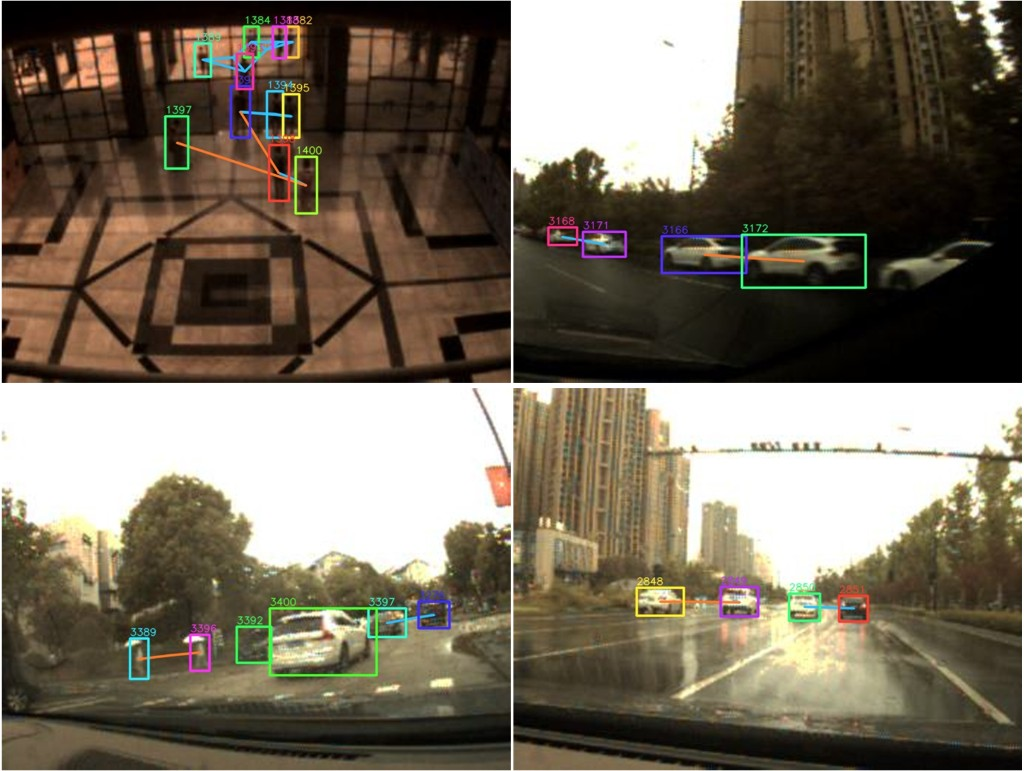
\includegraphics[width=\textwidth]{hyper-vis.png}
  \caption{Frame-level hypergraph on four FEMOT test frames. Cyan segments are spatial hyperedges and orange segments are RGB hyperedges.}
  \label{fig:hypervis}
\end{figure*}

Figure~\ref{fig:hypervis} draws the frame-level hypergraph on four FEMOT test frames. Each box is one track, and one identity keeps one color. A cyan segment joins a spatial hyperedge, whose member centers lie inside the normalized radius $0.10$. An orange segment joins an RGB hyperedge. That edge is built from the HyLA-enhanced block-1 descriptor when the cosine is at least $0.841$ and the two tracks are mutual top-$5$ neighbors.

On the driving frames the two relations fall on different pairs. Nearby cars share the spatial edge, and the RGB edge links a pair whose boxes sit farther apart but agree in appearance. The indoor frame is more crowded, so the two relations cross inside one group of people. A hyperedge aggregates that group. The pairwise row in the main paper replaces each such group by a two-endpoint edge.

\FloatBarrier

\end{document}
